% !TeX spellcheck = en_GB
\section{Intercultural Management}

\subsection{''Models'' of culture}

\subsubsection{Cultural Model}

The analogy of the iceberg helps us to understand the meaning of culture within an international setting that is characterized by high diversity. Only the tip of the iceberg is visible while the larger part below the surface escapes the eye.

\begin{figure}[H]
	\centering
	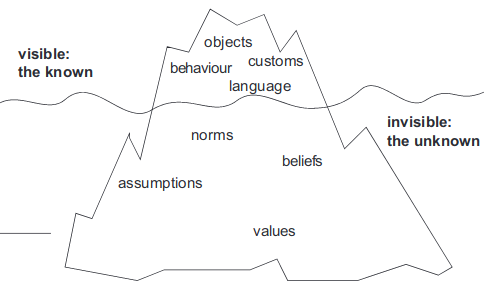
\includegraphics[width=0.8\textwidth]{figures/icebergCulture.png}
	\caption{The Iceberg as a cultural model}
\end{figure}

\subsubsection{Dune model of culture}

\begin{figure}[H]
	\centering
	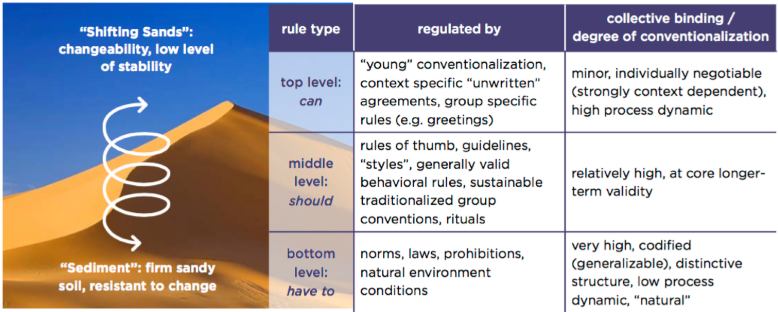
\includegraphics[width=\textwidth]{figures/duneModelCulture.png}
	\caption{The dune model of culture}
\end{figure}

\subsubsection{Six spheres of inclusion model (SSI Model, Onion Model)}
It ''is a tool that helps us to understand what is at play in any global diversity encounter, either interpersonal or organizational. It allows us to break out of a domestic diversity bias that might thwart the broader development of employees and the organization itself.''
\begin{figure}[H]
	\centering
	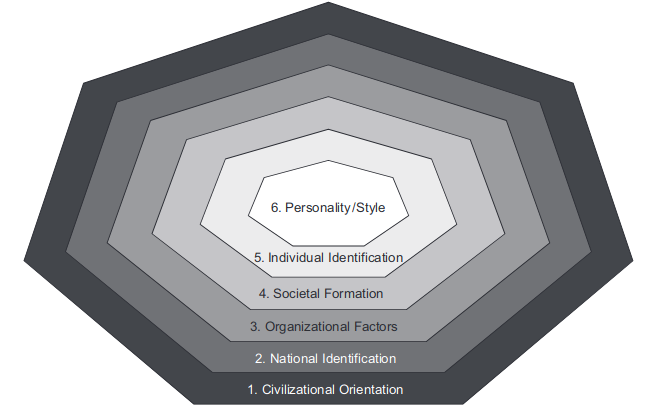
\includegraphics[width=.9\textwidth]{figures/ssiModelCulture.png}
	\caption{SSI or onion model}
\end{figure}
The context in which we are at any given moment determines which layer of the onion predominates. In South-East Asia for example, people from the West are primarily seen as Westerners, whereas in Great Britain we might be perceived as Swiss, German, or French. Other examples would be urban people, country folks, mountain people, Thurgovians, etc. All the layers influence the behaviour, the actions and feelings of a person and they stand in reciprocal relation. The layers civilization and nationality represent a kind of superstructure. The layers personality and individual represent the core, of which personal factors like gender, genes, skills and possibilities are examples. The layers society and organization are bridging the superstructure and the core.

\subsection{Stereotypes and generalization}
The distinction between stereotypes and generalizations is crucial to our perception and judgment of others. If we want to understand people from other cultures, we have to sharpen our perception in order to avoid stereotyping.

\subsubsection{Stereotype}
A cultural stereotype is the application of a generalization to every person in a cultural group.\\
E.g. Germans are aggressive.\\
Asians are always eating.

\subsubsection{Generalization}
Cultural generalizations search for \textbf{tendencies} in a group that shares certain values and beliefs and engages in certain patterns of behaviour. A tendency is an \textbf{average quality} or value and tries to be \textbf{objective and non-judgmental}.\\
E.g. Germans are not aggressive, they just have a more direct way of communication.\\
Lunch is an important part of the Asian culture.

\mbox{}\\
A generalization never fully applies to a culture, but it represents more or less the ''average'' of a culture.
\begin{figure}[H]
	\centering
	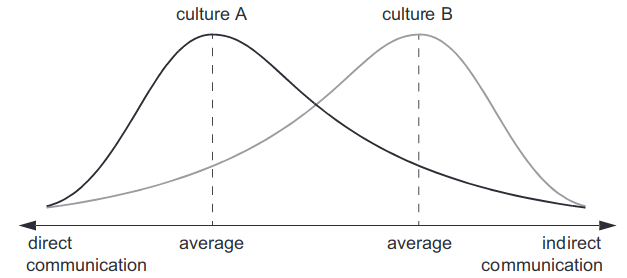
\includegraphics[width=.8\textwidth]{figures/culturalDistribution.png}
	\caption{Cultural generalization: Distribution according to communication styles}
\end{figure}

\subsection{Communication differences}

\subsubsection{Style of communication}

\paragraph{High and low context}
Context is the information that surrounds an event. The elements that combine to produce a given meaning – events and context – are in different proportions depending on culture. The cultures of the world can be compared on a scale from high to low context.
\begin{figure}[H]
	\centering
	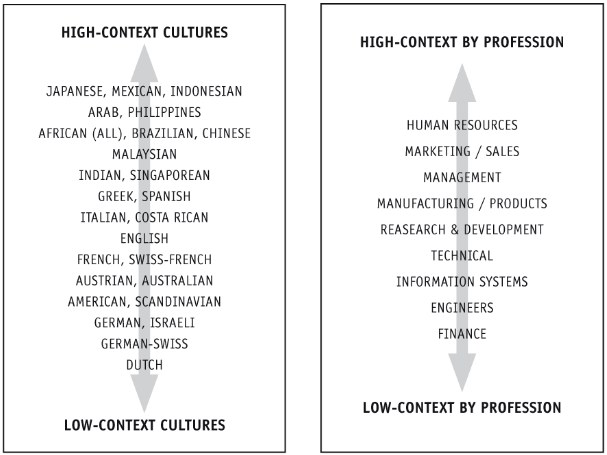
\includegraphics[width=.7\textwidth]{figures/contextComparison.png}
	\caption{Cultures and professions ordered by context}
\end{figure}
A High Context communication or message is one in which most of the information is already in the person, while very little is in the coded, explicit, transmitted part of the message. A Low Context communication is just the opposite; i.e., the mass of the information is vested in the explicit code.

\paragraph{Indirect and direct communication}
\begin{description}
	\tightlist
	\item[Direct] Meaning is conveyed through explicit statements made directly to the people involved, with little reliance on contextual factors such as a situation and timing.\\
	(What you see is what you get!)
	\item[Indirect] Meaning is conveyed by suggestion, implication, non-verbal behaviour, and other contextual cues; for instance, statements intended for one person may be made within earshot to a different person.\\
	(What you get is what you manage to see!)
\end{description}
\begin{figure}[H]
	\centering
	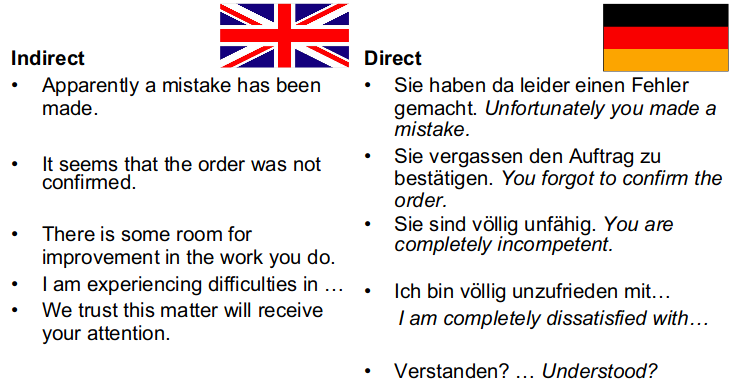
\includegraphics[width=.8\textwidth]{figures/indirectDirectCommunication.png}
	\caption{Some examples for indirect (English) vs. direct (German)}
\end{figure}

\paragraph{Low-scan and high-scan}
\begin{description}
	\tightlist
	\item[Low-scan] Meaning is conveyed predominantly through words. Low-scan people are often seen by high-scan communicators as „under-scanners“.\\
	(I have said it!)
	\item[High-scan] Meaning is conveyed through non-verbals, to time, to space, to hierarchy, gender, age, privilege etc. High-scan people are often seen by low-scan communicators as „over-scanners“.\\
	(He told it to me in the hall! You should have heard it, the way he said it! He looked directly into my eyes.)
\end{description}

\paragraph{Attached (involved) and detached communication}
\begin{description}
	\tightlist
	\item[Attached] Issues are discussed with feeling and emotion, conveying the speaker’s personal stake in the issue and the outcome.\\
	(If it’s important, it’s worth getting worked up over!)
	\item[Detatched] Issues are discussed with calmness and objectivity, conveying the speaker’s ability to weigh all factors impersonally.\\ (If it’s important, it shouldn’t be tainted by personal bias!)
\end{description}

\paragraph{Intellectual and relational confrontation}
\begin{description}
	\tightlist
	\item[Intellectual confrontaion] Disagreement with ideas is stated directly, with the assumption that only the idea, not the relationship, is being attacked.\\
	(We are just arguing – don’t take it personally!)
	\item[Relational confrontation] Relational issues and problems are confronted directly, while intellectual disagreement is handled more subtly and indirectly.\\
	(Be authentic about your feelings and respectful of other’s ideas!)
\end{description}

\paragraph{Abstract and concrete communication}
\begin{description}
	\tightlist
	\item[Abstract] Issues are best understood through theories, principles, and data, with emphasis on the general rather than the specific.\\
	(What’s the principle?)
	\item[Concrete] Issues are best understood through stories, metaphors, allegories, and examples, with emphasis on the specific rather than general.\\
	(What’s an example?)
\end{description}

\subsubsection{Patterns of silence}
For the Anglo-Saxons, when A stops, B starts. It is not polite to interrupt. The even more verbal Latins integrate slightly more than this; B will frequently interrupt A and vice versa to show how interested each is in what the other is saying.

The pattern of silent communication for oriental languages frightens the Westerner. The moment of silence is interpreted as a failure to communicate.

\begin{figure}[H]
	\centering
	\includegraphics[width=.8\textwidth]{figures/silencePatternsCommunication.png}
	\caption{Different styles of verbal communication}
\end{figure}

\subsubsection{Tone of voice}
Another crosscultural problem arises from the tone of voice. The figure below shows typical patterns for Anglo-Saxon, Latin and oriental languages. For some neutral societies, ups and downs in speech suggest that the speaker is not serious. But in most Latin societies this „exaggerated“ way of com-municating shows that you have your heart in the matter. Oriental societies tend to have a much more monotonous style; self-controlled, it shows respect. Frequently, the higher the position a person holds, the lower and flatter their voice.

\subsection{Seven dimensions of culture}

\subsubsection{Universalism vs. Particularism}
Whether a culture is based on rules and standards (universalism) or relationship and trust (particularism).

\begin{tabularx}{\textwidth}{X|X}
	Universalism & Particularism \\ 
	\hline 
	Focus is more on rules than relationships. & Focus is more on relationships than on rules. \\ 
	Legal contracts are readily drawn up. & A trustworthy person is the one who honours changing mutualities. \\ 
	There is only one truth or reality, that which has been agreed to. & There are several perspectives on reality relative to each participant. \\ 
	A deal is a deal & Relationships evolve \\ 
\end{tabularx}

\subsubsection{Individualism vs. Collectivism}
Whether a culture focuses more on the group or individual.

\begin{tabularx}{\textwidth}{X|X}
	Individualism & Collectivism \\ 
	\hline 
	More frequent use of “I” form. & More frequent use of “We” form. \\ 
	Decisions made on the spot by representative & Decisions referred back by delegate to organisation \\ 
	People ideally achieve alone and assume personal responsibility & People ideally achieve in groups which assume joint responsibility \\ 
	Vacations taken in pairs, even alone & Vacations in organised groups or extended families \\ 
\end{tabularx}

\subsubsection{Specific vs. Diffuse}
Whether the public and private life are closely linked (diffuse) or not (specific).

\begin{tabularx}{\textwidth}{X|X}
	Specific & Diffuse \\ 
	\hline 
	Direct, to the point, purposeful in relating. & Indirect, circuitous, seemingly “aimless” forms of relating. \\
	Precise, blunt, definitive and transparent. & Evasive, tactful, ambiguous, even opaque. \\ 
	Principles and consistent moral stands independent of the person being addressed. & Highly situational morality depending upon
	the person and context encountered. \\ 
\end{tabularx}

\subsubsection{Neutral vs. Affective}
Whether the person within a culture expresses one's emotion openly (affective) or not (neutral).

\begin{tabularx}{\textwidth}{X|X}
	Neutral & Affective \\ 
	\hline 
	Do not reveal what they are thinking or	feeling. & Reveal thoughts and feelings verbally and non-verbally. \\ 
	May (accidentally) reveal tension in face and posture. & Transparency and expressiveness release tensions. \\ 
	Emotions often dammed up will occasionally explode. & Emotions flow easily, effusively, vehemently and without inhibition. \\ 
	Cool and self-possessed conduct is admired. & Heated, vital, animated expressions admired. \\ 
	Physical contact, gesturing or strong facial expressions often taboo. & Touching, gesturing and strong facial expressions common. \\
	Statements often read out in monotone. & Statements declaimed fluently and dramatically. \\
\end{tabularx}

\subsubsection{Achievement vs. Ascription}
Whether a culture rewards according to one's performance or one's age, status or gender.

\begin{tabularx}{\textwidth}{X|X}
	Achievement oriented & Ascription oriented \\ 
	\hline 
	Use of titles only when relevant to the competence you bring to the task. & Extensive use of titles, especially when these clarify your status in the organisation. \\ 
	Respect for superior in hierarchy is based on how effectively his or her job is performed and how adequate their knowledge. & Respect for superior in hierarchy is seen as a measure of your commitment to the organisation and its mission. \\ 
	Most senior managers are of varying age and	gender and have shown proficiency in specific	jobs. & Most senior managers are male, middle-aged and qualified by their background. \\ 
\end{tabularx}

\subsubsection{Sequential time vs. synchronous time}
Whether people tend to do one thing at a time (sequential) or several things at one (synchronous).

\begin{tabularx}{\textwidth}{X|X}
	Sequential & Synchronous \\ 
	\hline 
	Only do one activity at the time. & Do more than one activity at the time. \\
	Time is sizeable and measurable. & Time is there; flexible time-management. \\ 
	Keep appointments strictly; schedule in advance and do not run late. & Schedules are generally subordinate to relationships. \\
	Strong preference for following initial plans. & Strong preference for following where relationships lead. \\
\end{tabularx}

\subsubsection{Internal direction vs. external direction}
To what extend do we control our environment or does the environment control us?

\begin{tabularx}{\textwidth}{X|X}
	Internal control & External control \\ 
	\hline 
	Often dominating attitude bordering on aggressiveness towards environment. & Often flexible attitude, willing to compromise and keep the peace. \\
	Conflict and resistance means that you have	convictions. & Harmony and responsiveness, that is, sensibility. \\ 
	Focus is on self, function, own group and own organisation. & Focus is on “other”, that is customer, partner, colleague. \\
	Discomfort when environment seems “out of control” or changeable. & Comfort with waves, shifts, cycles if these are “natural”. \\
\end{tabularx}

\subsection{Relationship to time}
There are three types of cultures with different relationships to time:

\begin{description}
	\tightlist
	\item[present-oriented] Relatively timeless, traditionless and ignores the future.
	\item[past-oriented] Mainly concerned to maintain and restore traditions in the present.
	\item[future-oriented] Envisaging a more desirable future and setting out to realise it.
\end{description}

\begin{tabularx}{\textwidth}{X|X|X}
	Past & Present & Future \\ 
	\hline 
	Talk about history, origin of family, business and nation. & Activities and enjoyments of the moment are most important. & Much talk of prospects, potentials, aspirations, future achievements.\\
	Motivated to recreate a golden age. & Plans not objected to, but rarely executed. & Planning and strategising done enthusiastically. \\ 
	Show respect for ances-tors, predecessors and older people. & Show intense interest in the present relationships “here and now”. & Show great interest in the youthful and in future potentials. \\
	Everything viewed in the context of tradition and history. & Everything viewed in terms of its contemporary impact and style. & Present and past, used, even exploited, for future advantage \\
\end{tabularx}

\subsection{The developmental model of intercultural sensitivity (DMIS)}
\begin{figure}[H]
	\centering
	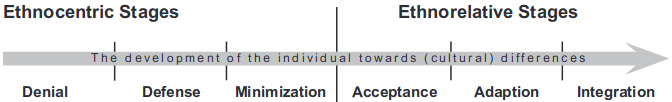
\includegraphics[width=\textwidth]{figures/DMISmodel.png}
	\caption{Different stages of the DMIS model}
\end{figure}

\subsubsection{Ethnocentric stages}
There are three ethnocentric stages. Being in one of these stages means that one’s own culture is experienced as central to reality in some way.

\begin{description}
	\tightlist
	\item[Denial] Denial of cultural difference is the state in which one’s own culture is experienced as the only real one. Other cultures are avoided by maintaining psychological and/or physical isolation from differences.
	\item[Defense] Defense against cultural differences is the state in which one’s own culture (or an adopted culture) is experienced as the only good one. The world is organized into “us and them”, where “we” are su-perior and “they” are inferior.
	\item[Minimization] Minimization of cultural difference is the state in which elements of one’s own cultural view are experienced as universal. Because these absolutes obscure deep cultural differences, other cultures may be trivialized or romanticized.
\end{description}

\subsubsection{Ethnorelative stages}
There are three ethnorelative stages. Being in one of these stages means that one’s own culture is experienced in the context of other cultures.

\begin{description}
	\item[Acceptance] Acceptance of cultural difference is the state in which one’s own culture is experienced as just one of a number of equally complex worldviews. Acceptance does not mean agreement – cultural difference may be judged negatively – but the judgment is not ethnocentric.
	\item[Adaption] Adaptation to cultural difference is the state in which the experience of another culture yields percepti-on and behaviour appropriate to that culture. One’s worldview is expanded to include constructs from other worldviews.
	\item[Integration] Integration of cultural difference is the state in which one’s experience of self is expanded to include the movement in and out of different cultural worldviews.
\end{description}

\subsection{Culture in the workplace}
In the context of the culture in the workspace the following dimensions can be analysed.

\subsubsection{Power distance}
\begin{tabularx}{\textwidth}{X|X}
	\textbf{Low} & \textbf{High} \\ 
	\hline 
	\begin{itemize}
		\tightlist
		\item Democtratic management style
		\item Power is not usually jealously guarded
		\item Decision making tends to be consultative
		\item Manager/subordinate relations are fairly informal
		\item Rank has few privileges
	\end{itemize}
	&
	\begin{itemize}
		\tightlist
		\item Authoritarian
		\item Power is centralized
		\item Decisions are made at the top
		\item Manager/subordinate relations are formal
		\item Rank has its privileges
	\end{itemize} \\
\end{tabularx}


\subsubsection{Attitude toward uncertainty}
\begin{tabularx}{\textwidth}{X|X}
	\textbf{Positive} & \textbf{Skeptical} \\ 
	\hline 
	\begin{itemize}
		\tightlist
		\item People are not afraid of talking risks or of failing
		\item Trial and error/experimenting is how we learn and improve our products and services
		\item Change is positive
		\item What we don’t know can’t hurt us.
	\end{itemize}
	&
	\begin{itemize}
		\tightlist
		\item Taking risks and failing have strong negative consequences and should be avoided if at all possible
		\item One doesn’t try something until one knows it will work
		\item Change is threatening
		\item What we don’t know can be troubling.
	\end{itemize} \\
\end{tabularx}

\subsubsection{Attitude toward work}
\begin{tabularx}{\textwidth}{X|X}
	\textbf{Achievement} & \textbf{Quality of life} \\ 
	\hline 
	\begin{itemize}
		\tightlist
		\item People are motivated by achievement
		\item Being successful means moving up,	getting ahead, and having greater power and responsibility
		\item One lives to work
	\end{itemize}
	&
	\begin{itemize}
		\tightlist
		\item A better quality of life is what motivates people to work
		\item a pleasant work setting and good relations with coworkers are as motivating as the chance to make more money and move up
		\item One works to live
	\end{itemize} \\
\end{tabularx}

\subsubsection{Key to productivity}
\begin{tabularx}{\textwidth}{X|X}
	\textbf{Results} & \textbf{Harmony} \\ 
	\hline 
	\begin{itemize}
		\tightlist
		\item Focusing on the task ensures success what matters	most in employees is their productivity and output, which are related to technical skills and experience
		\item conflict is sometimes necessary to clear the air and move forward
		\item getting results is ultimately more important than how you get them
		\item employee loyalty is not as important as performance/productivity
	\end{itemize}
	&
	\begin{itemize}
		\tightlist
		\item Harmony in the Workplace ensures the success of an organization
		\item Conflict should be minimized because of disruptive consequences
		\item How you get results is as important as the results themselves
		\item Loyalty is expected and reciprocal
	\end{itemize} \\
\end{tabularx}

\subsubsection{Source of status}
\begin{tabularx}{\textwidth}{X|X}
	\textbf{Achieved} & \textbf{Ascribed} \\ 
	\hline 
	\begin{itemize}
		\tightlist
		\item Rank,	status, and respect must be	earned and do not come with the position or title
		\item People are respected and promoted based on their performance
		and achievements, regardless of age or seniority
		\item People of higher rank/status should not act superior to/better than those of lesser.
	\end{itemize}
	&
	\begin{itemize}
		\tightlist
		\item Rank, position, and title confer auto-
		matic status and respect
		\item Achievements are important for promotion, but age and seniority are also highly valued
		\item People should be careful not to behave above/below their station in life.
	\end{itemize} \\
\end{tabularx}

\subsection{Culture shock}

\subsection{Resolving conflicting values}